\documentclass{beamer}

\usepackage{pgf}
\usepackage{tikz}

\title{Fun with glibc's runtime linker}
\author{Marvin Blauth}

\begin{document}

\frame{\titlepage}

\begin{frame}
  \frametitle{The rtld has parameters!}
  \begin{itemize}
    \item The rtld can be used as executable, e.g. /lib64/ld-2.23.so
    \item For the dynamically linked rtld environment variables can be used, e.g. LD\_LIBRARY\_PATH
  \end{itemize}
\end{frame}

\begin{frame}
  \frametitle{Interesting rtld environment variables}
  \begin{itemize}
    \item LD\_BIND\_NOW -- Force resolving of all symbols on startup
    \item LD\_PRELOAD -- Preload symbols from selected library
    \item LD\_DEBUG -- Print debug information for linker activity
    \item LD\_AUDIT -- Register an audit library to be invoked on linker activity
    \item There are many more options, check out \textbf{man ld.so}
  \end{itemize}
\end{frame}

\begin{frame}
  \frametitle{LD\_AUDIT}
  \begin{itemize}
    \item glibc's implementation was based on the auditing interface present on Solaris
    \item The auditing interface enables you to register symbols to be called on almost any step of the linker activity
    \item Example: When searching for a symbol in a shared library lib.so, the symbol \textbf{la\_objsearch} will be
          called with "lib.so" as parameter.
  \end{itemize}
\end{frame}

\begin{frame}
  \frametitle{Using LD\_AUDIT for fun and profit}
  \begin{itemize}
    \item The auditing interface can not just monitor the linker activity, but also reject it
    \item This can be used for performing any sort of actual audit on the linker activity, for instance
    \begin{itemize}
      \item OSS license compatibility
      \item Library file checksum
      \item Installation source of library
    \end{itemize}
  \end{itemize}
\end{frame}

\begin{frame}
  \frametitle{Using LD\_AUDIT for checking the installation source 1/2}
  \begin{itemize}
    \item Imagine you want your software to only use symbols from the system repositories
    \item LD\_AUDIT in combination with libhawkey/libhif/libdnf lets you very easily do that on Fedora
  \end{itemize}
\end{frame}

\begin{frame}
  \frametitle{Using LD\_AUDIT for checking the installation source 2/2}

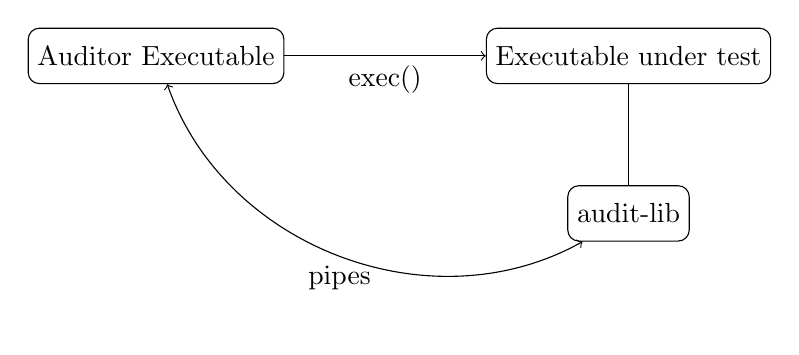
\begin{tikzpicture}
  \tikzset {
    box/.style={
      rectangle,
      rounded corners,
      draw=black,
      minimum height=2em,
      text centered
    }
  }
  \node[box](auditor) {Auditor Executable};
  \node[box, right of=auditor, node distance=6cm](exec) {Executable under test};
  \node[box, below of=exec, node distance=2cm](lib) {audit-lib};

  \path (auditor) edge[->] node[anchor=south,below]{exec()} (exec);
  \path (exec) edge (lib);
  \path (lib) edge[<->,bend left=50] node[anchor=south,below]{pipes} (auditor);

\end{tikzpicture}

\end{frame}

\end{document}